%!TEX root = ..\..\Main.tex
\chapter{Teori}

\section{A* Algoritmen}

A* er en algoritme til at beregne den korteste rute baseret på en række heuristiske datasæt. A* får input igennem en brugerlavet graf der indeholder en række datasæt for at algoritmen kan fungere.  Først har vi distancen fra punkt til punkt, eksempelvis punkt 'A' til punkt 'B' som vi kalder for f.eks. \textbf{'H'} og dernæst har vi et datasæt \textbf{'G'} der indeholder bekostningen for at flytte fra en kant til en anden, denne variabel er bestemt på forhånd. Et virkelighedseksempel kunne være at man vil over på den anden side af en sø, så har man så muligheden for at svømme direkte eller gå uden om og det koster f.eks. 2 gange så meget at bevæge sig direkte igennem søen. \cite{trafikoekonomi}

\vspace{5mm}

En måde man kan visualisere A* på er f.eks. med et kvadrat-system som set i figur \ref{A*Kvadrat-1}. Her kan vi se at vi har et start punkt (grøn) og et slutpunkt (blå). De kvadrater vi ikke kan bevæge os igennem er de røde kvadrater. Figuren angiver ingen heuristiske datasæt endnu, så derfor har den ikke videre funktionalitet, fordi A* algoritmen som sagt modtager data igennem en graf.

\begin{wrapfigure}{l}{0.60\textwidth}
    \centering
    \includegraphics[width=0.60\textwidth]{Pictures/Teoriafsnit/Figurfiler/Grid1.png}
    \caption{Kvadrat-system}
    \label{A*Kvadrat-1}
\end{wrapfigure}

Primært når det kommer til belægning af en dynamisk rute, foregår det ved at en enhed fortsætter hen i mod et mål indtil den når en forhindring. Dette er et ekstremt simpelt bevægelsesmønster og indebærer in vis in-effektivitet. Rent retorisk kunne man stille spørgsmålet om det ikke ville være smartere at planlægge en rute før man overhovedet bevæger sig.